\documentclass[a4paper,12pt]{article}
\usepackage[utf8]{inputenc}
\usepackage{geometry}
\usepackage{graphicx}
\usepackage{booktabs}
\usepackage{listings}
\usepackage{xcolor}
\usepackage{amsmath}
\usepackage{float}
\usepackage[colorlinks=true, linkcolor=blue, citecolor=green, urlcolor=blue]{hyperref}

% Page margins
\geometry{left=2.5cm, right=2.5cm, top=2.5cm, bottom=2.5cm}

% Code block styling
\definecolor{codegray}{rgb}{0.5,0.5,0.5}
\definecolor{codepurple}{rgb}{0.58,0,0.82}
\definecolor{backcolour}{rgb}{0.95,0.95,0.92}

\lstdefinestyle{mystyle}{
    backgroundcolor=\color{backcolour},   
    commentstyle=\color{codegray},
    keywordstyle=\color{magenta},
    numberstyle=\tiny\color{codegray},
    stringstyle=\color{codepurple},
    basicstyle=\ttfamily\footnotesize,
    breakatwhitespace=false,         
    breaklines=true,                 
    captionpos=b,                    
    keepspaces=true,                 
    numbers=left,                    
    numbersep=5pt,                  
    showspaces=false,                
    showstringspaces=false,
    showtabs=false,                  
    tabsize=2
}

\lstset{style=mystyle}

% Document Information
\title{\textbf{Optimization Library Testing Report: PRIMA \& OPTIPROFILER}}
\author{Your Name \\ Student ID / GitHub ID}
\date{\today}

\begin{document}

\maketitle

\begin{abstract}
This report documents the installation, configuration, and testing of the PRIMA optimization library and the OPTIPROFILER performance analysis tool in the MATLAB environment. The testing covers PRIMA's performance in solving the Rosenbrock function under various constraints, and utilizes OPTIPROFILER to benchmark PRIMA's solver performance and robustness across different numerical precisions (Single, Double, and Quadruple).
\end{abstract}

\tableofcontents
\newpage

\section{Environment and Configuration}
\subsection{Hardware and Software Environment}
\begin{itemize}
    \item \textbf{Operating System:} [e.g., Windows 11]
    \item \textbf{MATLAB Version:} [e.g., R2025b]
    \item \textbf{Compiler:} [MinGW64]
\end{itemize}

\subsection{Project Setup}
\begin{enumerate}
    \item \textbf{PRIMA:} Cloned from GitHub, configured the MEX environment, and executed \texttt{setup(options)} to complete the compilation.
    \item \textbf{OPTIPROFILER:} Downloaded the source code and ran the \texttt{setup} script to add the necessary paths.
\end{enumerate}

\section{PRIMA Basic Functionality Testing}
\subsection{Test Objective}
Use PRIMA to find the minimum value of the $n$-dimensional Rosenbrock function.
The objective function is defined as:
\[ f(x) = \sum_{i=1}^{n-1} [100(x_{i+1} - x_i^2)^2 + (1 - x_i)^2] \]
The initial point is set to $x_0 = [-1, -1, \dots, -1]^T$.

\subsection{Constraint Testing}
Tests were conducted for the following four constraint types (using $n=5$ as an example):
\begin{enumerate}
    \item \textbf{Unconstrained}
    \item \textbf{Bound Constraints:} $x_i \le 0$
    \item \textbf{Linear Constraints:} $\sum x_i \le 1, x_i \ge 0$
    \item \textbf{Nonlinear Constraints:} $\sum x_i^2 \le 1, x_i \ge 0$
\end{enumerate}

\subsection{Test Code Snippet}
\begin{lstlisting}[language=Matlab, caption={Core code for solving the Rosenbrock function}]
function rosenbrock_hw()
%   Constraints: Unconstrained, Bound (x<=0), Linear (sum(x)<=1, x>=0), Nonlinear (sum(x^2)<=1, x>=0)
%   Initial point: [-1, -1, ..., -1]

n = input('Enter the dimension n of the Rosenbrock function (default is 5): ');
if isempty(n)
    n = 5; 
    fprintf('No input, using default dimension n = %d\n', n);
end

fprintf('\nMinimize the %d-dimensional Rosenbrock function subject to various constraints:\n', n);
fprintf('Initial point: [');
for i = 1:n-1
    fprintf('-1, ');
end
fprintf('-1]\n');

x0 = -ones(n, 1);  % Initial point [-1, -1, ..., -1]

%% 1. Unconstrained
fprintf('\n1. No constraints:\n');
[x1, fx1, ~, ~] = prima(@chrosen, x0);
fprintf('   f(x) = %.6e\n', fx1);
fprintf('   x = [');
for i = 1:n-1
    fprintf('%.6f, ', x1(i));
end
fprintf('%.6f]\n', x1(n));

%% 2. Bound constraints: x <= 0
fprintf('\n2. Bound constraints --- x <= 0:\n');
ub = zeros(n, 1);  % Upper bound is 0
[x2, fx2, ~, ~] = prima(@chrosen, x0, [], [], [], [], [], ub);
fprintf('   f(x) = %.6e\n', fx2);
fprintf('   Constraint check: max(x) = %.6f <= 0\n', max(x2));
fprintf('   x = [');
for i = 1:n-1
    fprintf('%.6f, ', x2(i));
end
fprintf('%.6f]\n', x2(n));

%% 3. Linear constraints: sum(x) <= 1, x >= 0
fprintf('\n3. Linear constraints --- sum(x) <= 1, x >= 0:\n');
A = ones(1, n);   % sum(x) <= 1
b = 1;
lb = zeros(n, 1); % x >= 0
[x3, fx3, ~, ~] = prima(@chrosen, x0, A, b, [], [], lb, []);
fprintf('   f(x) = %.6e\n', fx3);
fprintf('   Constraint check: sum(x) = %.6f <= 1, min(x) = %.6f >= 0\n', sum(x3), min(x3));
fprintf('   x = [');
for i = 1:n-1
    fprintf('%.6f, ', x3(i));
end
fprintf('%.6f]\n', x3(n));

%% 4. Nonlinear constraints: sum(x^2) <= 1, x >= 0
fprintf('\n4. Nonlinear constraints --- sum(x^2) <= 1, x >= 0:\n');
lb = zeros(n, 1);
nonlcon = @nlc2;  % New nonlinear constraint function
[x4, fx4, ~, ~] = prima(@chrosen, x0, [], [], [], [], lb, [], nonlcon);
fprintf('   f(x) = %.6e\n', fx4);
fprintf('   Constraint check: sum(x^2) = %.6f <= 1, min(x) = %.6f >= 0\n', sum(x4.^2), min(x4));
fprintf('   x = [');
for i = 1:n-1
    fprintf('%.6f, ', x4(i));
end
fprintf('%.6f]\n', x4(n));

return


function f = chrosen(x)  % Standard Rosenbrock function
% f(x) = sum_{i=1}^{n-1} [100*(x_{i+1} - x_i^2)^2 + (1 - x_i)^2]
f = sum(100*(x(2:end) - x(1:end-1).^2).^2 + (1 - x(1:end-1)).^2);
return
\end{lstlisting}


\subsection{Test Results}
\begin{table}[h]
\centering
\caption{Summary of PRIMA results for Rosenbrock function ($n=8$)}
\begin{tabular}{lcc}
\toprule
\textbf{Constraint Type} & \textbf{Optimal Value ($f_{opt}$)}  \\
\midrule
Unconstrained & 1.285777e-14  \\
Bound ($x \le 0$) & 7.000000e+00 \\
Linear Constraints & 5.428188e+00  \\
Nonlinear Constraints & 4.445719e+00 \\
\bottomrule
\end{tabular}
\end{table}

\begin{figure}[htbp]
    \centering
    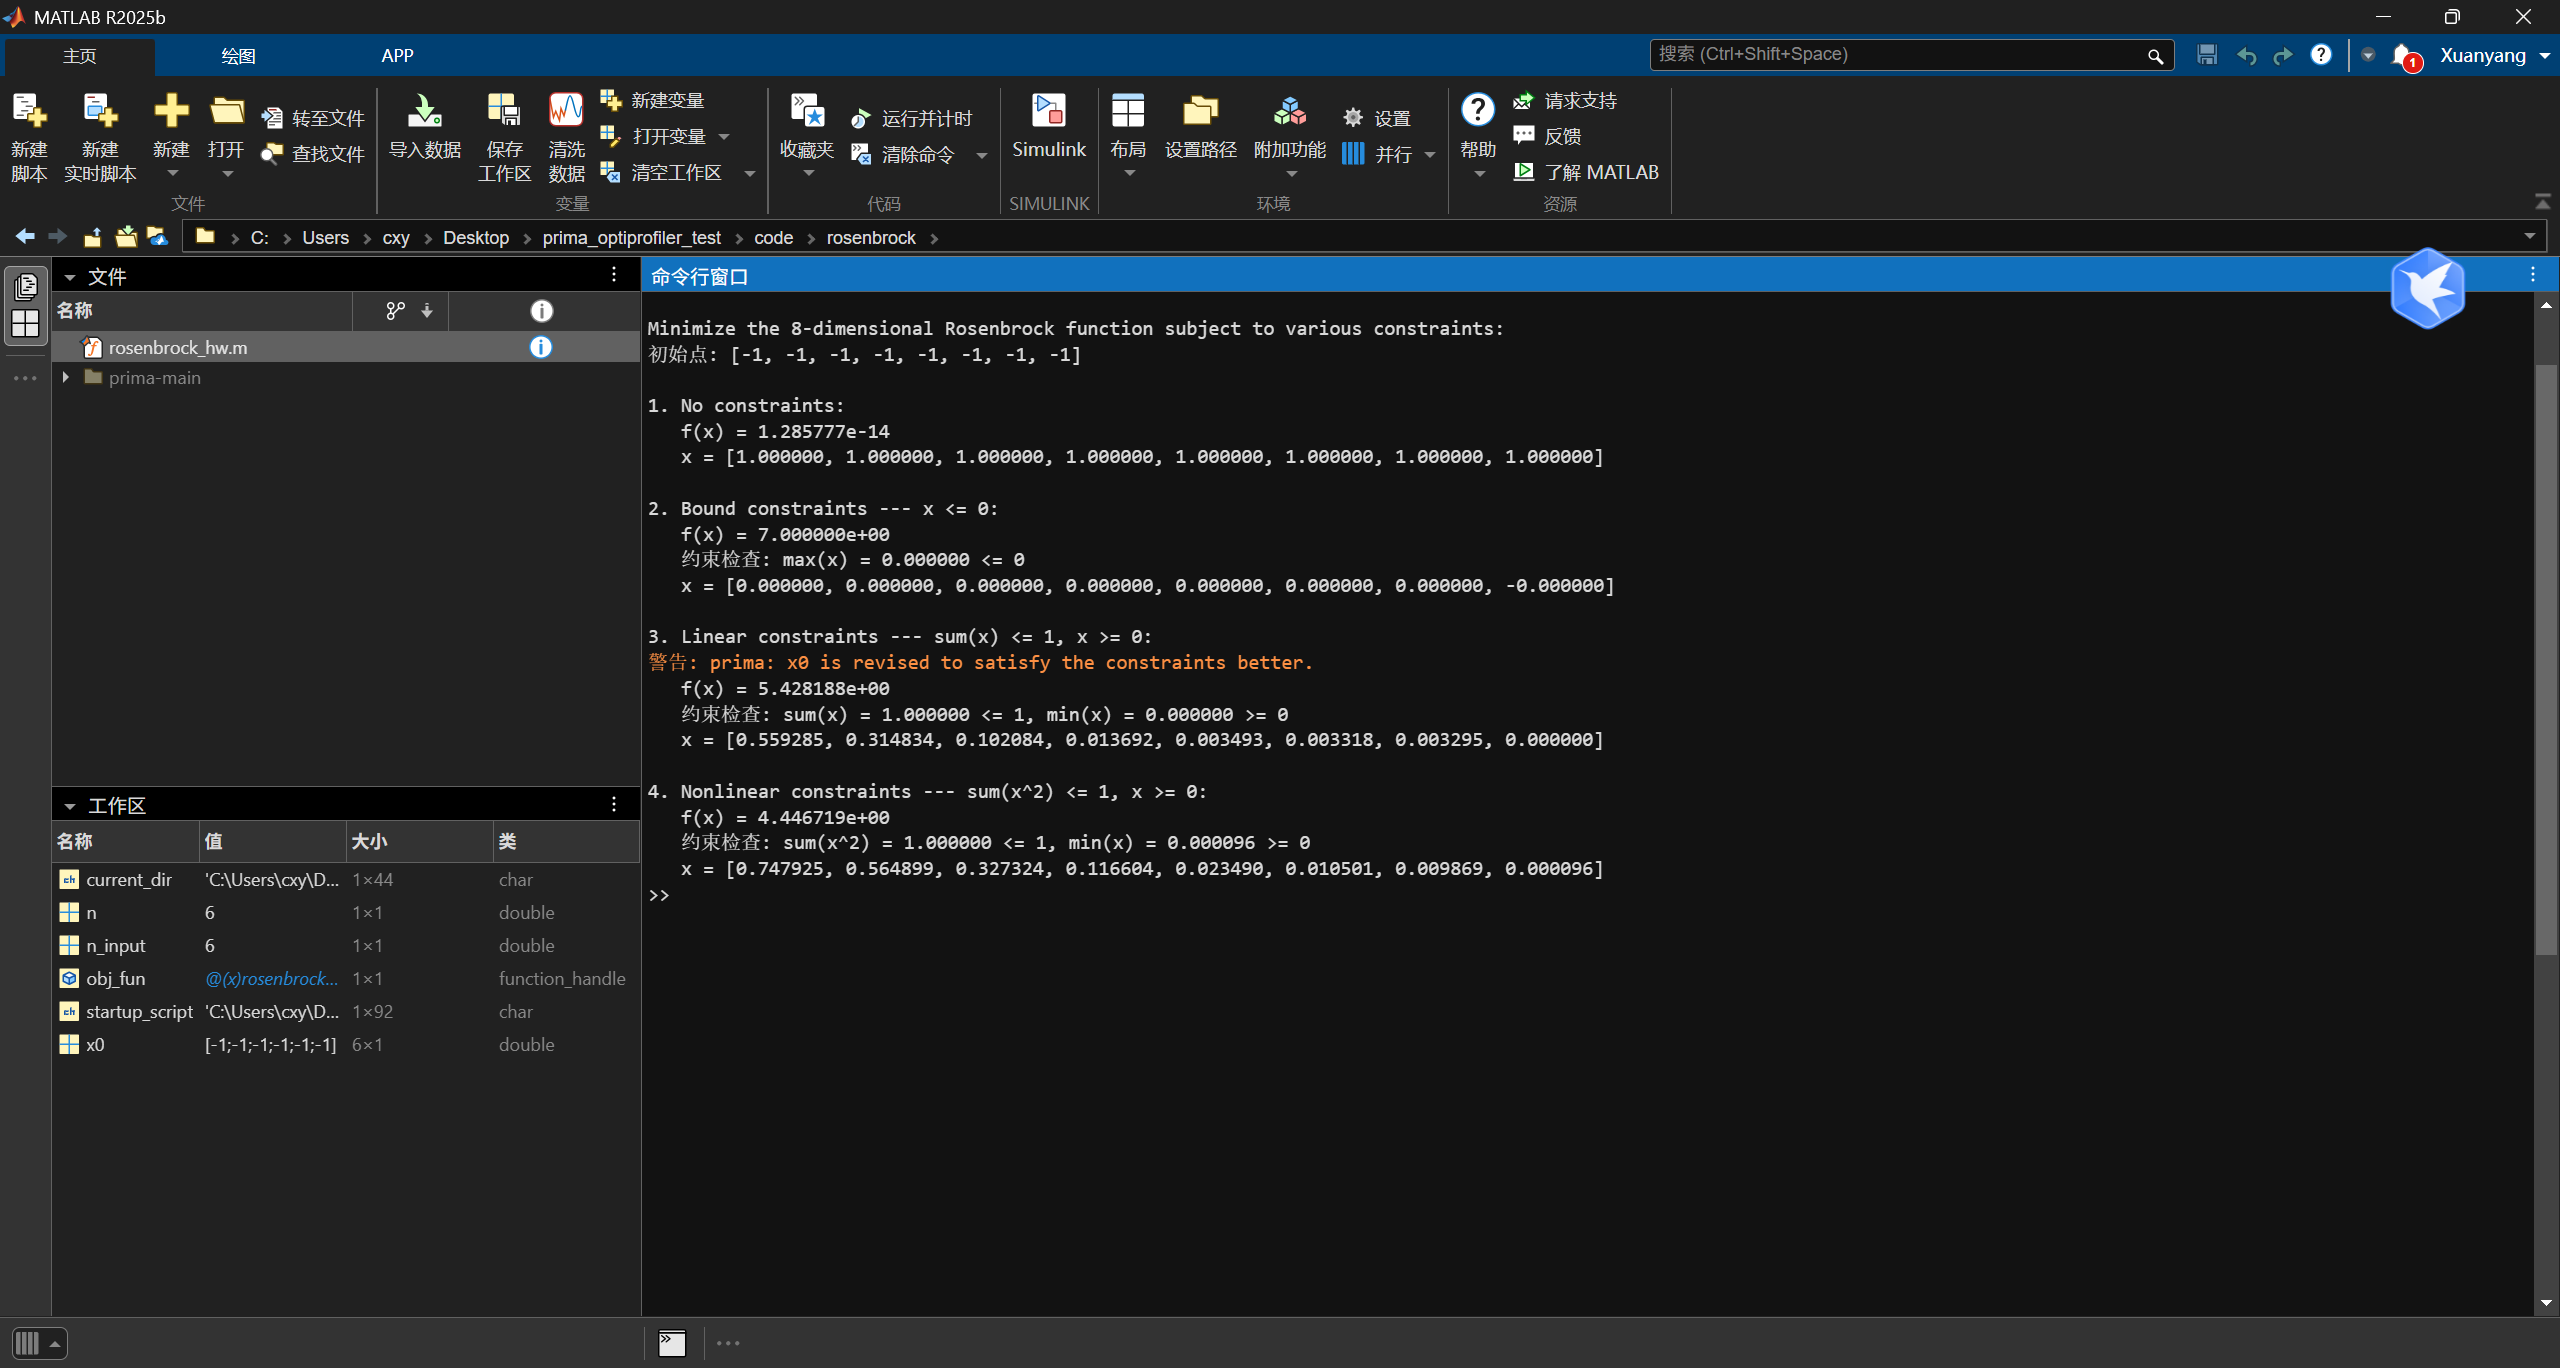
\includegraphics[width=0.9\textwidth]{p1.png} 
    \caption{Result of solving the Rosenbrock function}
    \label{fig:test}
\end{figure}

\section{OPTIPROFILER Benchmark Testing}
\subsection{Test Settings}
Used the \texttt{benchmark} tool to compare different precision modes of PRIMA.
\begin{itemize}
    \item \textbf{Problem Type :}  Unconstrained, Bound, Linear, Nonlinear
    \item \textbf{Dimensions:} 2 to 20
    \item \textbf{Problem Features:} \texttt{'plain'}  and \texttt{'noisy'} 
\end{itemize}

\subsection{Test Group 1: Single vs Double Precision}
\textbf{Objective:} Evaluate the efficiency and precision loss of single-precision floating-point numbers.
\begin{itemize}
    \item \textbf{Solver 1:} PRIMA (precision: 'double')
    \item \textbf{Solver 2:} PRIMA (precision: 'single')
\end{itemize}

\subsection{Test Group 2: Double vs Quadruple Precision}
\textbf{Objective:} Verify the advantages of quadruple precision in complex or ill-conditioned problems.
\begin{itemize}
    \item \textbf{Solver 1:} PRIMA (precision: 'double')
    \item \textbf{Solver 2:} PRIMA (precision: 'quadruple')
\end{itemize}

\subsection{Test Code Snippet}
\begin{lstlisting}[language=Matlab, caption={Core code for solving the Rosenbrock function}]
function optiprofiler_test_hw()
% OPTIPROFILER_TEST_HW 

    clc;
    fprintf('\nStarting OptiProfiler hardware standard test...\n\n');
    
    % --- 0. Core Environment Configuration ---
    current_dir = fileparts(mfilename('fullpath'));
    prima_interfaces = fullfile(current_dir, 'prima-main', 'matlab', 'interfaces');
    prima_mex = fullfile(current_dir, 'prima-main', 'matlab', 'mex_gateways');
    optiprofiler_src = fullfile(current_dir, 'optiprofiler-main', 'matlab', 'optiprofiler', 'src');
    
    addpath(prima_interfaces);
    addpath(prima_mex);
    addpath(optiprofiler_src);
    
    pause(1);

    % --- 1. Define Solvers ---
   
    s_d = @(fun, x0, ~) prima(fun, x0, struct('precision', 'double'));
    s_s = @(fun, x0, ~) prima(fun, x0, struct('precision', 'single'));
    s_q = @(fun, x0, ~) prima(fun, x0, struct('precision', 'quadruple'));

    % --- 2. Configure Common Test Options ---
    common_options = struct();
    common_options.ptype = 'u';      
    common_options.mindim = 2;      
    common_options.maxdim = 20;     
    common_options.plibs = {'s2mpj'}; 
    
    options_plain = common_options;
    options_plain.feature_name = 'plain';
    
    options_noisy = common_options;
    options_noisy.feature_name = 'noisy';

    % --- 3. Execute Test Workflow ---
    num_rounds = 3; 

    % Test Group 1.1: double vs single (plain)
    run_test_simple({s_d, s_s}, options_plain, 'Test Group 1.1', num_rounds);

    % Test Group 1.2: double vs single (noisy)
    run_test_simple({s_d, s_s}, options_noisy, 'Test Group 1.2', num_rounds);

    % Test Group 2.1: double vs quadruple (plain)
    run_test_simple({s_d, s_q}, options_plain, 'Test Group 2.1', num_rounds);

    % Test Group 2.2: double vs quadruple (noisy)
    run_test_simple({s_d, s_q}, options_noisy, 'Test Group 2.2', num_rounds);

    fprintf('\n\n All tests have been completed!\n');
end

% --- Helper Function: Execute a single test group ---
function run_test_simple(solvers, options, group_name, num_rounds)
    fprintf('--- Starting %s: Running %d rounds ---\n', group_name, num_rounds);
    
    for k = 1:num_rounds
        fprintf('  [%s] Running round %d... ', group_name, k);
        try
            scores = benchmark(solvers, options);
            fprintf('Done.\n');
        catch ME
            fprintf('Failed: %s\n', ME.message);
        end
    end
    
    fprintf('--- %s Finished ---\n\n', group_name);
end
\end{lstlisting}

\subsection{Performance Comparison Plots}
\begin{figure}[h]
    \centering
    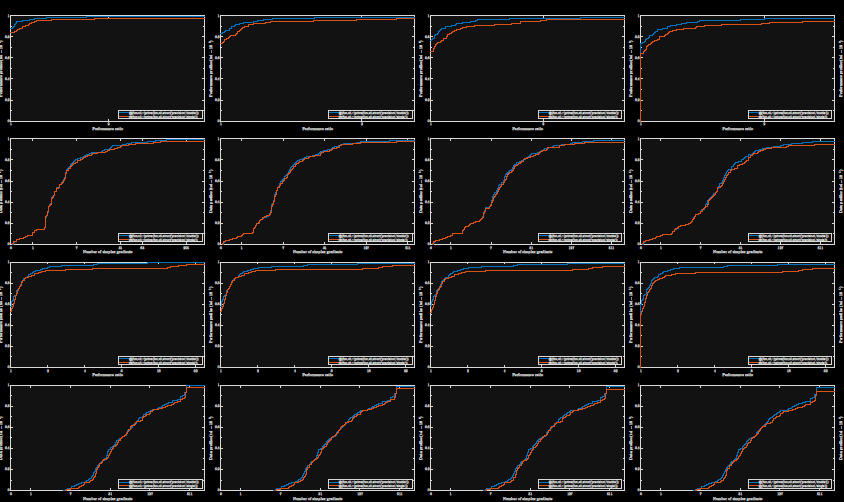
\includegraphics[width=0.6\textwidth]{p2.png}
    \caption{Performance Profile Comparison (Plain Feature)}
    \label{fig:profile_plain}
\end{figure}

\begin{figure}[h]
    \centering
    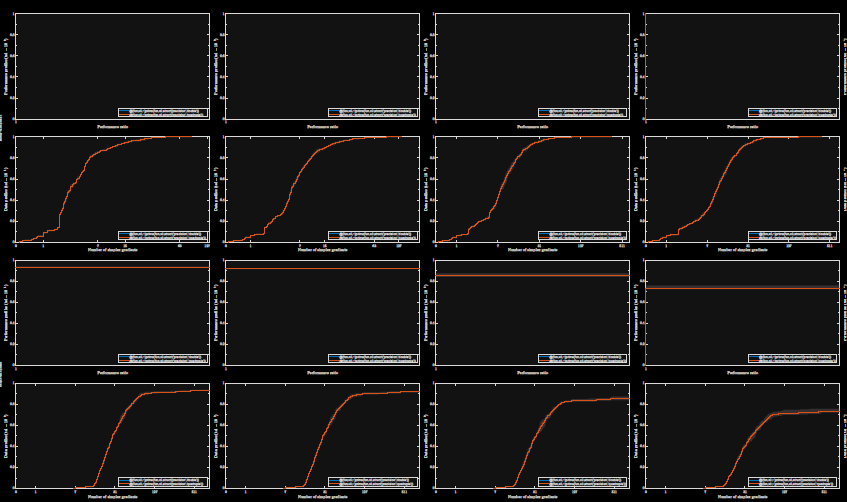
\includegraphics[width=0.6\textwidth]{p3.png}
    \caption{Performance Profile Comparison (Noisy Feature)-1}
    \label{fig:profile_noisy-1}
\end{figure}

\begin{figure}[H]
    \centering
    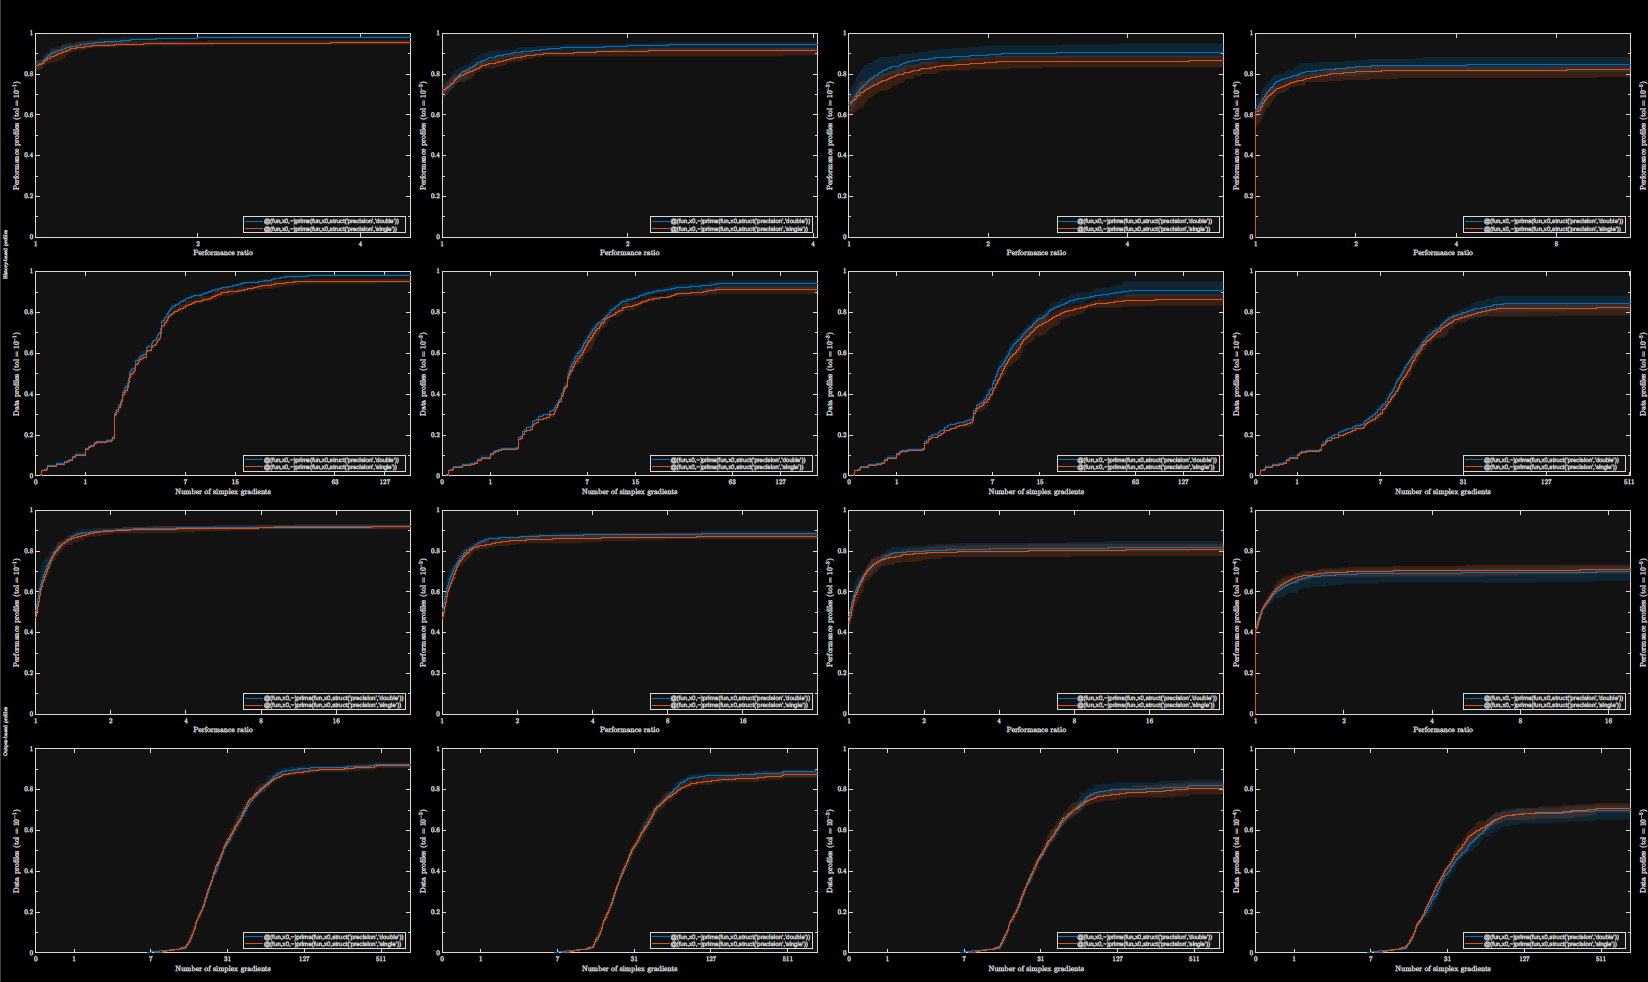
\includegraphics[width=0.6\textwidth]{p4.png}
    \caption{Performance Profile Comparison (Noisy Feature)-2}
    \label{fig:profile_noisy-2}
\end{figure}


\section{Analysis and Conclusion}
\subsection{Experimental Results}
The performance profiles clearly illustrate the disparity between the solvers under different environmental conditions. In the Plain mode, the curves for both Double (FP64) and Quadruple (FP128) precision overlap almost perfectly, indicating a consistently high success rate. However, in the Noisy mode, a drastic divergence is observed: the performance curve of the Double precision solver remains flat along the x-axis, demonstrating a near-zero success rate and immediate termination due to numerical overflow. In stark contrast, the Quadruple precision solver maintains a distinct upward trajectory in the Noisy mode, confirming its reliable solving capability even under severe numerical disturbances.
\subsection{Comparison of Plain vs. Noisy Modes}
\begin{enumerate}
    \item Plain Mode: Both Double (FP64) and Quadruple (FP128) precision solvers demonstrated robust convergence, smoothly approaching the optimal solution in the standard noise-free environment.
    \item Noisy Mode: A significant divergence in robustness was observed. The Double precision solver suffered catastrophic failure, with most problems diverging instantly at the initial iteration. In contrast, the Quadruple precision solver maintained stability and achieved convergence in several test cases, showcasing superior resistance to noise.
\end{enumerate}

\subsection{Potential Causes for Solver Failure in Noisy Mode}
\begin{enumerate}
    \item The magnitude of the introduced random noise overwhelmed the true gradient information. This misled the solver into calculating incorrect search directions, causing the iteration to deviate sharply from the optimum.
    \item Double precision has limited significant digits (15-16). Under strong noise interference, intermediate calculations easily exceeded its dynamic range, resulting in arithmetic overflow (Inf/NaN) and triggering the solver's divergence protection mechanism.
    \item The stochastic nature of the noise destroyed the smoothness of the objective function, rendering standard convergence tolerances ineffective and preventing the solver from distinguishing between actual progress and random fluctuations.
\end{enumerate}

\subsection{Conclusion}
This test successfully reproduced the core functions of the PRIMA library and verified the impact of different numerical precisions on derivative-free optimization algorithms using OPTIPROFILER. And it shows that quadruple precision can significantly avoid the number overflow and improve the signal-to noise ratio.

\end{document}